%% Template for EU report, using the report.sty style file

\documentclass[12pt,a4paper,twoside]{article}
%% common package
\usepackage[headers]{report}
\usepackage{xspace}
\usepackage{verbatim}
\usepackage[usenames]{color}
\usepackage[usenames,dvipsnames,table]{xcolor}
\usepackage[pdftex,dvips]{graphicx}
\usepackage{url}
\usepackage{array}
\usepackage{color}
\usepackage{longtable}
%%

%%insert here other packages needed by sections

%%

%%%%%%%%%%%%%%%%%%%%%%%%%%%%%%%%%%%%%%%%%%%%%%%%%%%%%%%%%%%%%%%%%%%%%%%%%%%%%%
%%% Titlepage
%%%%%%%%%%%%%%%%%%%%%%%%%%%%%%%%%%%%%%%%%%%%%%%%%%%%%%%%%%%%%%%%%%%%%%%%%%%%%%

% declaration of variables used in style
\reportDocnumber{Year 1}
\reportTitle{First year periodic report}

\reportAuthor{CoDyCo Consortium}
\reportResponsiblePartner{IIT}
\reportAffiliation{% Insert here authors affiliations
 IIT, TUD, UPMC, UB, JSI.
}

\reportReviewer{}
\reportCoordinator{Francesco Nori}
\reportActivityNumber{1} %% n=1,..,10
\reportActivity{RTD}
\reportDoctype{Periodic report} %% or Prototype
\reportClassification{Public} % or Consortium
\reportDistribution{Consortium} %
\reportStatus{Draft} % Draft or Final
\reportDeliveryDate{28/04/2014}
\reportVersion{1.0}
\reportDate{Apr.~28, 2014}
\reportYear{2014}
\reportPages{\pageref{LastPage}}
\reportChangelog{v.1.0 & Feb 13, 2013 & First draft %%\\\hline
%%              v.2.0 & Feb 20, 2007 & Final version
}
\reportProjectStartingDate{1st March 2013}
\reportProjectEndDate{28th February 2017}
\reportProjectAcronym{CoDyCo}
\reportProjectTitle{Whole-Body Compliant Dynamical Contacts in Cognitive Humanoids}
 \reportContractNumber{600716}
 \reportProjectCoordinator{Istituto Italiano di Tecnologia}
 \reportProjectUrl{www.codyco.eu}
 \reportFrameworkProgramme{FP7}
 
 \reportWorkpackage{All work packages}
 \reportEditors{Francesco Nori, Vincent Padois, Jan Peters, Jan Babic, Michael Mistry}
 \reportContributors{Entire CoDyCo consortium}
 \reportReviewers{-}
\reportAbstract{The scope of the current report is to present the results ...}
\reportReviewers{reviewers}
\reportKeywordList{kw, list, etc, }

%%%%%%%%%%%%%%%%%%%%%%%%%%%%%%%%%%%%%%%%%%%%%%%%%%%%%%%%%%%%%%%%%%%%%%%%%%%%%%
%%% Sections
%%%%%%%%%%%%%%%%%%%%%%%%%%%%%%%%%%%%%%%%%%%%%%%%%%%%%%%%%%%%%%%%%%%%%%%%%%%%%%

%% constants{}

%%%%%%%%%%%%%%%%%%%%%%%%%%%%%%%%%%%%%%%%%%%%%%%%%%%%%%%%%%%%%%%%%%%%%%%%%%%%%%
%%% Misc. by Vincent
%%%%%%%%%%%%%%%%%%%%%%%%%%%%%%%%%%%%%%%%%%%%%%%%%%%%%%%%%%%%%%%%%%%%%%%%%%%%%%
\usepackage{titlesec}
\newcommand{\sectionbreak}{}
\graphicspath{{./images/}}
\usepackage{pdfpages}
\usepackage{caption}
\usepackage{subcaption}
\usepackage{slashbox}
\usepackage{multirow}
\usepackage{appendix}
\usepackage{hyperref}
\hypersetup{
    bookmarks=true,         % show bookmarks bar?
    unicode=false,          % non-Latin characters in Acrobat’s bookmarks
    pdftoolbar=true,        % show Acrobat’s toolbar?
    pdfmenubar=true,        % show Acrobat’s menu?
    pdffitwindow=false,     % window fit to page when opened
    pdfstartview={FitH},    % fits the width of the page to the window
    pdftitle={yearReport.pdf},    % title
    pdfauthor={Vincent Padois},     % author
    pdfsubject={Year 1 report for the CODYCO project},   % subject of the document
    pdfcreator={Vincent Padois},   % creator of the document
    pdfproducer={Vincent Padois}, % producer of the document
    pdfkeywords= {}, % list of keywords
    pdfnewwindow=true,      % links in new window
    colorlinks=true,       % false: boxed links; true: colored links
    linkcolor=black,          % color of internal links (change box color with linkbordercolor)
    citecolor=black,        % color of links to bibliography
    filecolor=black,      % color of file links
    urlcolor=black           % color of external links
}

%%
%%%%%%%%%%%%%%%%%%%%%%%%%%%%%% BEGIN DOCUMENT
\begin{document}

\reportMaketitle


%%TODO move to style
\newcolumntype{L}[1]{>{\raggedright\let\newline\\\arraybackslash\hspace{0pt}}m{#1}}
\newcolumntype{C}[1]{>{\centering\let\newline\\\arraybackslash\hspace{0pt}}m{#1}}
\newcolumntype{R}[1]{>{\raggedleft\let\newline\\\arraybackslash\hspace{0pt}}m{#1}}

\textbf{Document Revision History}
\begin{center}
\begin{tabular}{|C{2cm}|C{3cm}|p{5cm}|C{4cm}|}
\hline
\textbf{Version}&\textbf{Date}&\textbf{Description}&\textbf{Author}\\\hline
First draft & date & description & author\\\hline
\end{tabular}
\end{center}
 
 \clearpage

\newpage
\renewcommand*\contentsname{Table of Contents}
\renewcommand*\listfigurename{Index of Figures}
\tableofcontents
\newpage
\listoffigures
\newpage

%%%%%%%%%%%%%%%%%%%%%%%% Start report content here.

\section{Project objectives for the period}

\subsection{Overview}

\emph{\color{red}[Please provide a short overview of the project objectives for the reporting period in question, as included in Annex I of the Grant Agreement. These objectives are required so that this report is a stand-alone document.]}

\begin{longtable}{|C{1.5cm}|C{1.5cm}|C{1.5cm}|C{2cm}|C{2cm}|C{2cm}|C{2cm}|}
\cline{1-6}
\footnotesize \textbf{Task}& \footnotesize \textbf{IIT}&\footnotesize \textbf{TUD}&\footnotesize \textbf{UPMC}& \footnotesize \textbf{JSI} &\footnotesize \textbf{UB} & \multicolumn{1}{l}{} \\ \hline
\footnotesize WP1 &  8.5    &  1    &  3     & -   & -     & \textbf{7}  \\  \hline
\footnotesize WP2 &  -        &  -     &  -       & 18 & 2.5 & \textbf{8}\\ \hline
\footnotesize WP3 &  6.58 & 4.6  &  22    & -    & -     & \textbf{13}\\ \hline
\footnotesize WP4 & -         & 8     &  3      & -   & -     & \textbf{12}\\ \hline
\footnotesize WP5 & -         & -      &  0.3   & -    & -     & \textbf{12}\\ \hline
\footnotesize WP6 & 2        & -      &  -        & -    & -     & \textbf{21}\\ \hline
\footnotesize WP7 & 1        & -      &  -        & -    & -     & \textbf{21}\\ \hline
\multicolumn{1}{l|}{}  & \textbf{26} & \textbf{26} & \textbf{26} & \textbf{23} & \textbf{24}  & \textbf{73} \\  \cline{2-7}
\end{longtable}

\subsubsection{WP1: toolbox for computing and controlling dynamics of whole-body movements with contacts (UB)}

\emph{\color{red}[Please provide a short overview of the work package 1 objectives for the reporting period in question, as included in Annex I of the Grant Agreement. These objectives are required so that this report is a stand-alone document.]}

\subsubsection{WP2: understanding and modelling human whole-body behaviours in physical interaction (JSI)}

There were three main objectives within WP2 for the first year of the project: (i) to thoroughly review and summarise the recent relevant literature on human postural control and whole body motion in contact with environment and/or human, and to define the protocols for experimental procedures, including obtaining ethics committee approval (Task 2.2), (ii) to work on designing of models for human whole body motion in contact where the aim was to form simplified models or high-level understanding of how additional supportive contacts affect human motor control strategies involved in balancing (Task 2.3), and (iii) to study the factors involved in human choice of contact utilization and to investigate how interaction through contacts can contribute to learning of whole body motor control (Task 2.3).

\subsubsection{WP3: control and optimization of whole-body motion in contact (UPMC)}

The objectives of WP3 for the first year of the project are threefold. The first one is to demonstrate the applicability of state of the art whole-body motion controllers, such as the one developed in \cite{salini2012} and \cite{delprete2013}, within the simulation tools evaluated and retained in WP1 and for simple rigid, multi-contact scenarios. The second one is to propose a formulation and a solver for the whole-body control problem at the reactive level that provides a more expressive, richer description of the control problem as well as an efficient way of solving it. The third one is to identify existing or potential ways of optimally coupling the local, reactive control level and the global, decision making one.

\subsubsection{WP4: adaptation, Generalization and Improvement of Compliant Control and Tasks with Contacts (TUD)}

The goal of WP4 is to endow the CoDyCo humanoid robot control architecture with the core abilities for the
adaptation, generalization and self-improvement of both control laws and tasks that involve physical interaction
with humans, and the environment. In this context, we propose learning approaches that work in conjunction
with the control architecture devised in WP3 and rather complement analytical robotic approaches with on-policy
learning than starting from scratch. A core idea behind this work package is that Learning should complement
classical approaches and not supersede them.

The first year objectives of WP4 include:
\begin{itemize}
 \item Fast regression methods that can deal with well structured input noise, such that physical models can
be learned and adapted for tasks that involve many uncertain contacts. A particular focus will be given to
prediction-based switching model.
% \item Approaches for immediate reward-based control model learning with uncertain state will be devised to ensure
% robust execution with online adaptation. Such approaches allow for learning operational space control laws with
% multiple compliant contacts.
% \item Novel methods for imitation and reinforcement learning of skills with contact will be devised and tested. These
% methods are based on hierarchical relative entropy policy search approaches (Daniel et al., 2012) and will be
% used both for learning tasks the local controllers of WP3.
\item Learning how to combine elementary tasks by imitation and reinforcement learning. The combinations involved
include the learned simultaneous use of elementary tasks, the sequential use as well as the co-articulation of
tasks.
\end{itemize}


\subsubsection{WP5: systems integration, standardization and evaluation on the iCub robot (IIT)}

The first year main objective for WP5 was the implementation of a validation scenario consisting of the balancing on different type of rigid contacts. The goal was to include multiple contact positions: feet, hands, back, buttocks, arms and legs. 


\subsubsection{WP6: management (IIT)}

The first year management was primarily dedicated to the project starting. Among the main goals the release of a project software repository.


\subsubsection{WP7: dissemination and Exploitation (IIT)}

The main dissemination objectives for the CoDyCo first year were the creation of a CoDyCo database infrastructure, a CoDyCo project website and participation to dissemination events towards academia and industry. 

\section{Work progress and achievements during the period}

\subsection{Progress overview and contribution to the research field}

\emph{\color{red}[Please provide a concise overview of the progress of the work and situate the main achievements in the context of the research field, including a comparative assessment with the current state of the art.]}

\subsubsection{WP1: toolbox for computing and controlling dynamics of whole-body movements with contacts (UB)}

\emph{\color{red}[Please provide a concise overview of the progress of the work and situate the main achievements in the context of the research field, including a comparative assessment with the current state of the art.]}

\subsubsection{WP2: understanding and modelling human whole-body behaviours in physical interaction (JSI)}

After the first year of project, all planed objectives have been reached and one experimental modification has been implemented.

A thorough review was created with summary of the recent literature on human postural control and whole body motion in contact with environment. It includes relevant publications up to date and reviews the methods for evaluation of postural stability of bipedal systems beyond available reviews \cite{Mergner2007, Azevedo2007}. The review provides a solid bridge in methodologies and terminologies used by the project partners from multi-disciplinary backgrounds. Based on the overall objectives of the project and the specific objectives of WP2, experimental setup was created and procedures were defined. We obtained ethics committee approval for all project related human experiments (approved by National Medical Ethics Committee of Republic of Slovenia, reference number 112/06/13).

We performed an experimental study and examined functional role of supportive hand contact at different locations where balance of an individual was perturbed by translational perturbations of the support surface. We examined the effects of handle location, perturbation direction and perturbation intensity on the postural control and the forces generated in the handle. We found that an additional supportive hand contact significantly reduced the maximal displacement of the subject's centre of pressure (CoP) regardless of the position of the handle, direction of the perturbation and its intensity. This is in agreement with the accepted belief that an additional hand contact with support in general reduces the destabilizing effect of balance perturbation \cite{Maki1997, Bateni2005, Maki2006, Wing2011}. On the other hand, the position of the handle had no effects on the maximal CoP displacement. This supports the idea that maintaining postural stability is the task of the highest priority and that the central nervous system does whatever necessary to keep the body balanced \cite{Winter1995}. Our findings are in contrast with the recent findings of Sarraf et al. \cite{Sarraf2014}. We submitted a manuscript explaining the results of our study to Gait \& Posture Journal. The manuscript is under review after minor revision and is expected to be published by the end of 2014 \cite{Babic2014}.

Most of the human studies that examine postural control \cite{Horak1986, Henry1998, Dimitrova2004} (including our above mentioned study) utilize one-time support perturbations that unpredictably perturb the balance of an individual. During our experiments we noticed that human subjects reacted to all such perturbations regardless of how small or slow the perturbation was or what was the initial acceleration of the perturbation. Our conclusion was that these reactions are essentially protective reactions that do not necessarily have counterbalancing effects \cite{McIlroy1995, Corbeil2013}. Such reactions mask the real factors involved in human choice of contact utilization. We therefore altered the perturbation methods for our further experiments and designed continuous perturbations in a frequency band that corresponds with typical human motion during postural control \cite{Nawayseh2006}.


\subsubsection{WP3: control and optimization of whole-body motion in contact (UPMC)}

After one year of project, the level of achievement of the objectives in WP3 meets the expectations.

The whole-body control frameworks developed by J. Salini and A. Del Prete as part of their respective PhD thesis \cite{salini2012}, \cite{delprete2013} have been tested for simple rigid, multi-contact scenarios in the XDE \cite{XDE} and Gazebo \cite{Gazebo} physics simulators. These two simulators have been retained in WP1 (Deliverable 1.1) as modular simulation frameworks dedicated to the evaluation of the control strategies in CODYCO.

In the meantime, a novel "Generalized Smooth Hierarchical Control" algorithm has been developed \cite{liu2013}. It offers a rich way of describing and solving multi-task problems under constraints: both strict and soft tasks hierarchies can be enforced, tasks can be inserted and removed in a continuous manner and their priorities can be switched smoothly. It appears as a potential alternative to recent work in this domain \cite{escande2012}. Alternatively, TUD has worked on a Bayesian optimization framework dedicated to the bipedal locomotion gait optimization \cite{calandra2014}, \cite{calandra2014b}.

Regarding the exploration of the potential ways of coupling the local, reactive control level and the global, decision making one, several works have been initiated mostly related to the generation of "globally optimal" reference trajectories to be tracked reactively by the local controller. The contributions in this domain over the first year of project are mostly related to the work of A. Ibanez \cite{ibanez2013}, \cite{ibanez2014-icra} and \cite{ibanez2014-ark}. The distributed MPC approach developed in this work tackles the locomotion and balance problem from a new perspective that shares similarities with recent contributions such as \cite{mordatch2012} where an optimization framework enables an automated generation of rich contact behaviors, and \cite{ott2013} that combines a kinesthetic teaching task with an algorithm partially inspired by our approach to improve the balancing behavior during interactions. In the meantime, TUD investigated the interchange of forces during cooperative tasks between humans and robots \cite{berger2013}.

\subsubsection{WP4: adaptation, generalization and improvement of compliant control and tasks with contacts (TUD)}

The goal of WP4 is to endow the CoDyCo
humanoid robot control architecture with the
core abilities for the adaptation, generalization
and self-improvement of both control laws and
tasks that involve physical interaction with
humans, and the environment.
During the first year, developed a novel 
probabilistic movement primitive representation that
can be used for imitation learning and for superimposing multiple motor tasks. 
TUD also started to investigate to predict the partner's behavior in 
human robot interaction scenarios. 

\subsubsection{WP5: systems integration, standardization and evaluation on the iCub robot (IIT)}

The first year WP5 activities have concentrated on the first year validation scenario. A complete description of the scenario can be found in ``D5.1 Scientific report on validation scenario 1: balancing on multiple rigid contact points.'' which discusses the technical implementation of the first year validation scenario (see \url{https://github.com/robotology-playground/codyco-deliverables/tree/master/D5.1/pdf}). With respect to the state of the art the work progress represents an implementation of well established torques controlled whole-body control strategies. The integration of tactile feedback within the whole-body controller is a peculiarity of the implemented CoDyCo validation scenario and therefore represent a step forward with respect to the current state of the art. At the moment of writing the current deliverable the iCub tactile sensors cover the feet, the torso, the arms and the hands and the implemented validation scenario accounts for contacts at the hands and feet.

\subsubsection{WP6: management (IIT)}

The CoDyCo project started successfully. Management activities included the definition of an amendment procedure smoothly organized by the consortium and the project officer. A software repository (\url{https://github.com/robotology/codyco}) was set up using state of the art versioning tools (git) and social coding website (\url{https://github.com}). 

\subsubsection{WP7: dissemination and exploitation (IIT)}

Within WP7, CoDyCo first year achievement include: dissemination at relevant academic and industrial events; realization of a CoDyCo experiment database to disseminate robot and humans datasets. 

\subsection{Work package 1 progress}

\subsubsection{System dynamics estimation software. Extension to
environmental compliance estimation (T1.4)}

During year one, TUD started to investigate the learning of dynamic models with
discontinuities. A new Gaussian process (GP) model was developed
that is explicitly designed to deal with non-linearities
induced through contacts with the environment. An example of such non-linearities 
and the approximated model reconstruction is shown in Figure \ref{fig:example_discontinuities}.
We called the developed supervised learning method manifold GP (mGP), as it 
jointly learns a transformation of the data into a feature space, and a GP regression 
 from the feature space to observed space. In future work, this promising approach 
 will be applied to motor skill learning task on the iCub with multiple contacts. 
 A preprint of this work was published this year [Calandra, R. and Peters, J. and Rasmussen, C. and Deisenroth,
M., 2014].

\begin{figure}
\centering
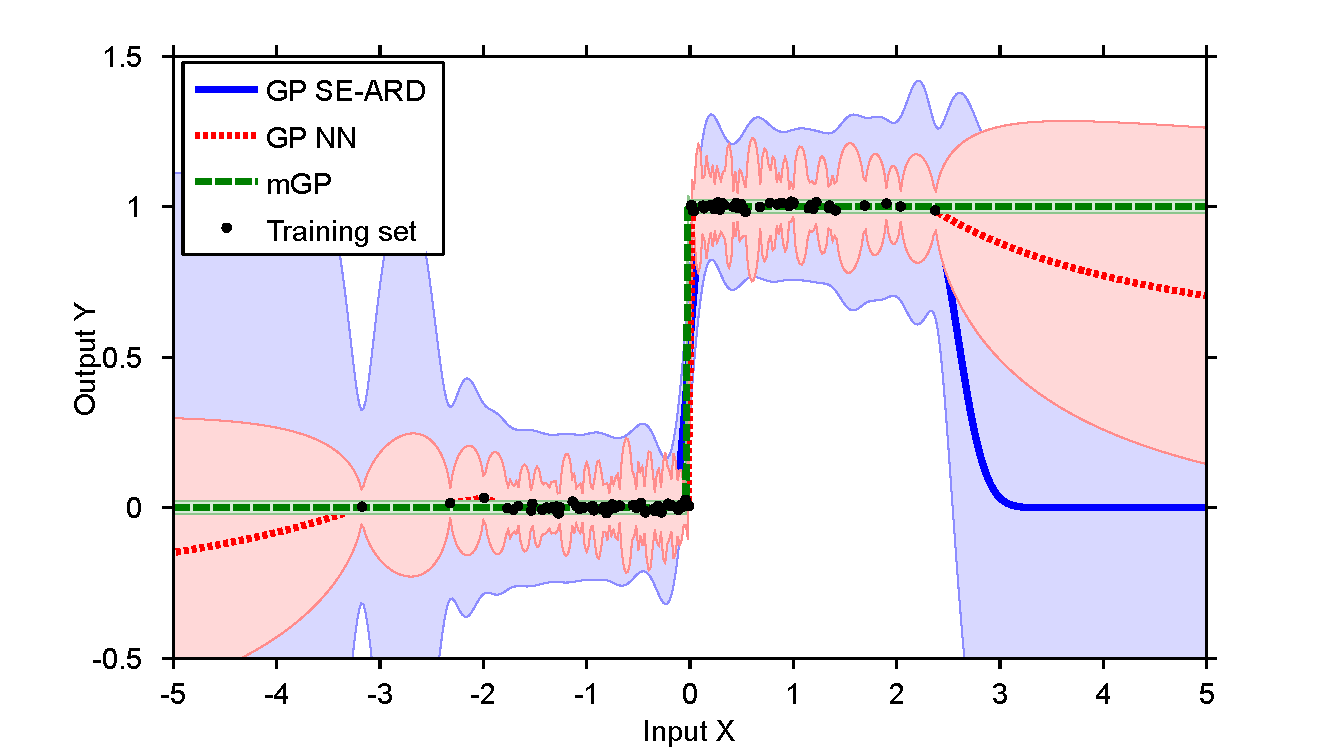
\includegraphics[width=0.7\textwidth]{./images/AAAI2014_0.pdf}
%\label{fig:subfig2}
 \caption{Illustration of a discontinuous function (black dots) that is approximated by three 
 model learning approaches. Classical Gaussian process regression methods (GP SE-ARD, and GP NN) 
 poorly reconstruct this function as they average over the ``jump'', which results in a high model variance. 
 TUD, however, demonstrated that by jointly learning a transformation of the data into a feature space, 
 and a GP regression model from the feature space to observed space, the non-linear function 
 can be reconstructed without large reconstruction errors. 
}
\label{fig:example_discontinuities}
\end{figure}

\subsubsection{Simulator for whole-body motion with contacts (T1.2)}

During year one, UPMC has led several activities related to the simulation of whole-body motion with contacts. These activities are described in deliverable 1.1 and can be summarized as follows:
\begin{itemize}
	\item definition of the requirements for the simulation framework;
	\item survey of the existing simulators for robotics \footnote{http://arxiv.org/abs/1402.7050};
	\item comparison between the XDE and Gazebo iCub simulators and a real iCub performing a free-falling task.
\end{itemize}

\emph{\color{red}[For work package 1 (UB) provide the following information:]}

\begin{itemize}
\item[-] \emph{\color{red}[A summary of progress towards objectives and details for each task;]}
\item[-] \emph{\color{red}[Highlight clearly significant results;]}
\item[-] \emph{\color{red}[If applicable, explain the reasons for deviations from Annex I and their impact on other tasks as well as on available resources and planning;]}
\item[-] \emph{\color{red}[If applicable, explain the reasons for failing to achieve critical objectives and/or not being on schedule and explain the impact on other tasks as well as on available resources and planning (the explanations should be consistent with the declaration by the project coordinator) ;]}
\item[-] \emph{\color{red}[a statement on the use of resources, in particular highlighting and explaining deviations between actual and planned  person-months per work package and per beneficiary in Annex 1 (Description of Work);]}
\item[-] \emph{\color{red}[If applicable, propose corrective actions.]}
\end{itemize}

\subsection{Work package 2 progress}

\subsubsection{Definition and design of experimental protocols (T2.1)}

The aim of the work in this task was to provide a solid multidisciplinary base for future research work within CoDyCo. We made a thorough review and summary of the recent relevant literature on human postural control and whole body motion in contact with environment (Delivery 2.1). The review examines postural control strategies without and with additional support contacts, types of perturbations that are commonly used to study neuromuscular functions involved in postural control and reviews the methods for stability evaluation of bipedal systems. The review is concluded with examination of stability metrics that can be applied for non-planar contacts. We plan to extend the review with methods of determination of inertial parameters of human/robot body and submit it for publication in a robotic journal by the end of 2014.

At JSI, we created an experimental setup to study human postural control and whole body motion in contact with environment. We implemented two state-of-the-art methods for perturbation of balance as shown on Figure \ref{fig:exp_protocol_W2} that will allow us to gain understanding how human brain deals with environment in the sense of supportive contacts. Using the same setup we can also validate all biomechanical findings on robotic systems by simply substituting the human subject with a robot. Besides, work has been undertaken to setup experiments also at UB. New equipment (the Moog Hapticmaster robot) was acquired and configured at both JSI and UB. Hapticmaster robot will be used in experiments with compliant and unpredictable contacts.

\begin{figure}
\centering
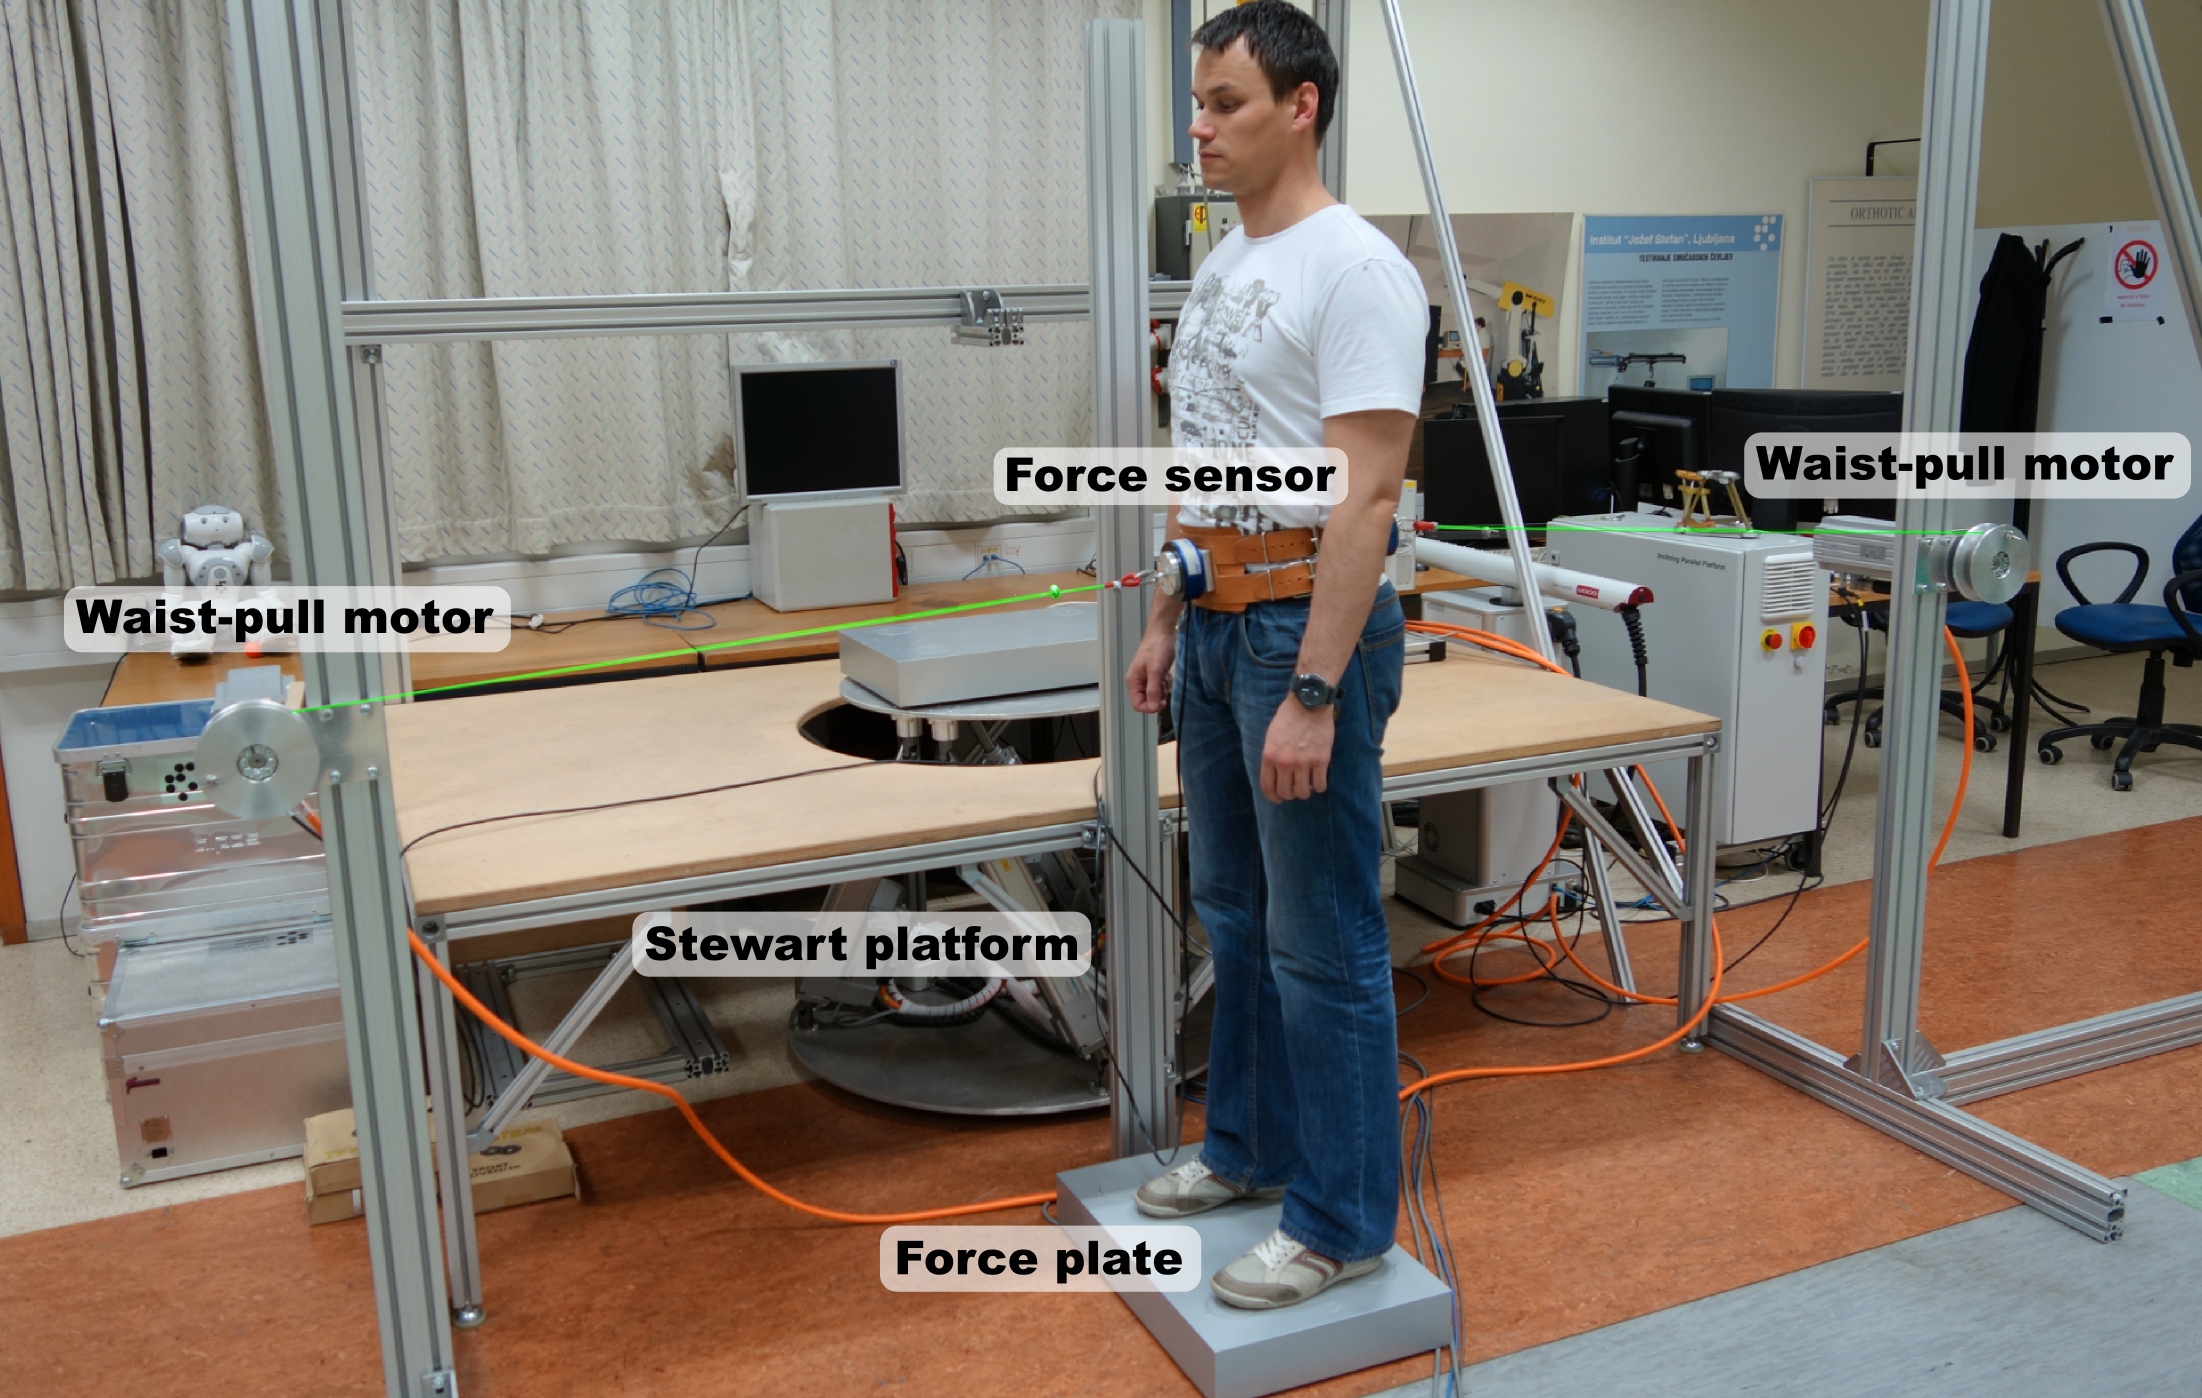
\includegraphics[width=0.8\hsize]{images/exp_setup_WP2.png}
\caption{Experimental setup to study human postural control and whole body motion in contact with environment. Front and back waist-pull motors together with the two force sensors located at the subject's waist allow real-time force perturbations of the subject while the Stewart platform can perturb the balance by either translational or rotational motion (or a combination of both) of the support surface. Force plates are used in combination with kinematical and electromiographical measurements (not on the figure) to study the adaptation of subjects to the given perturbations.}
\label{fig:exp_protocol_W2}
\end{figure}

\subsubsection{Design of models for human whole body motion in contact (T2.2)}

Work has begun on understanding how to derive simplified models of whole-body balance that will encapsulate the task relevant parameters of posture control with multiple contacts. By emulating situations when balance of an individual is challenged, we examined functional role of supportive hand contact at different locations where balance of an individual was perturbed by translational perturbations of the support surface. The experimental methods rested upon our work in Task 2.1 and are depicted on the left side of Figure \ref{fig:exp_paper_W2}.

\begin{figure}
\centering
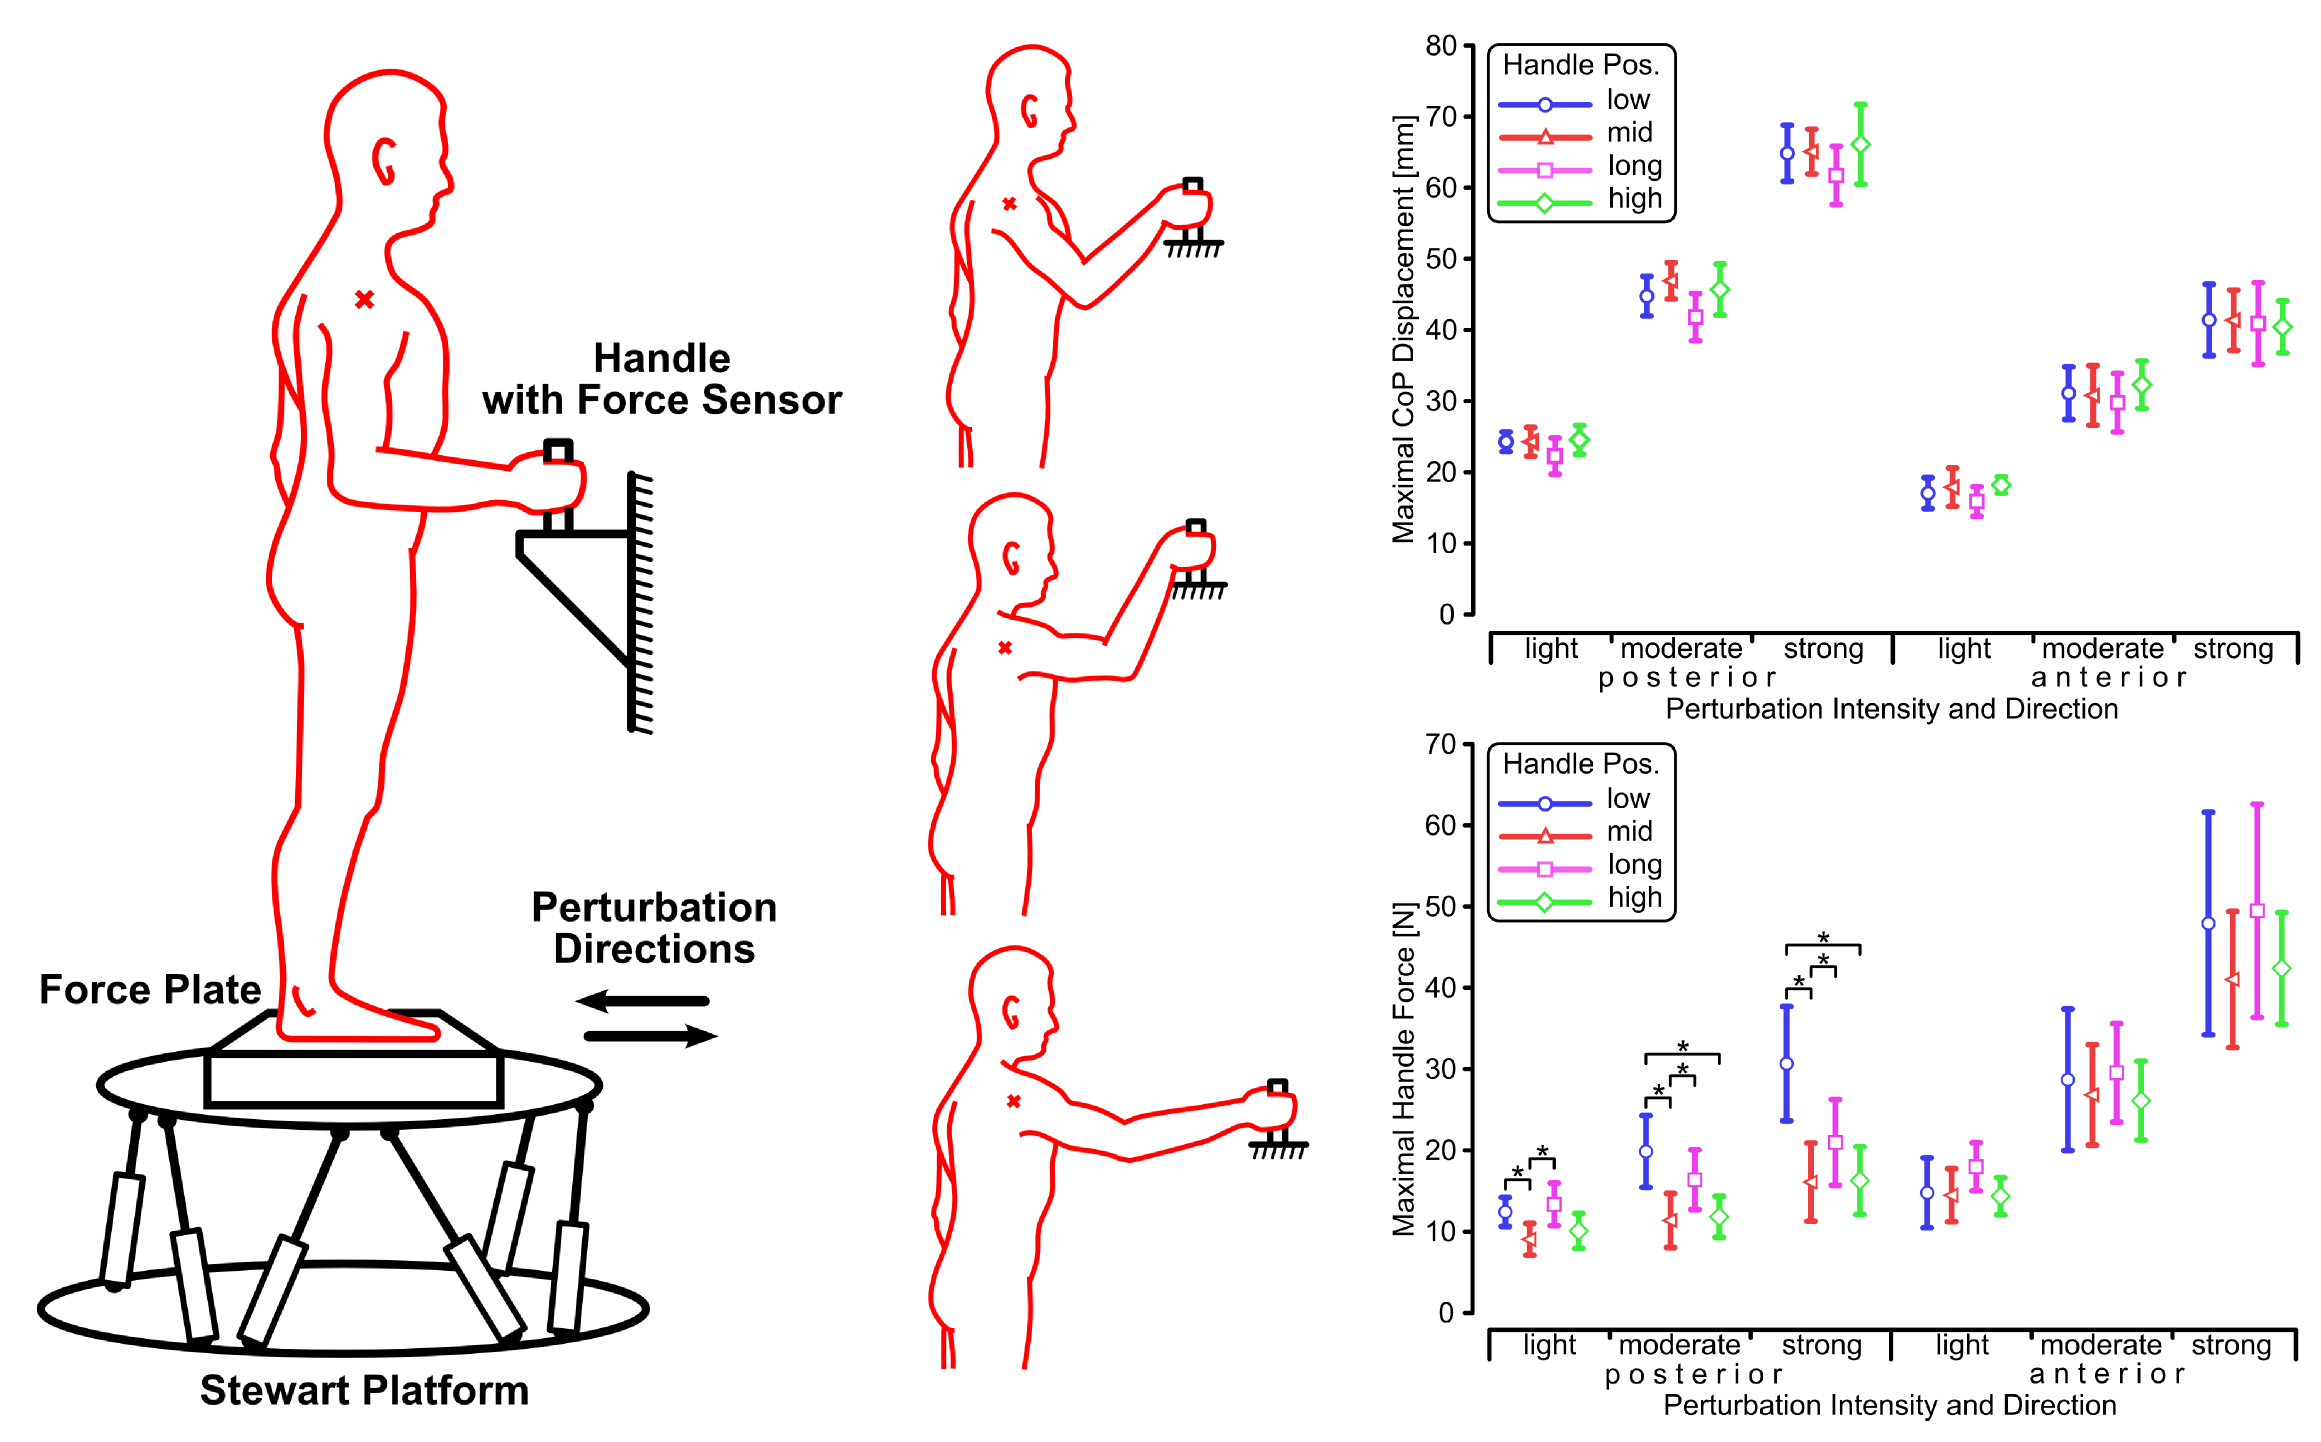
\includegraphics[width=0.8\hsize]{images/exp1_JSI.png}
\caption{Examining functional role of supportive hand contact. The subjects were standing on a force plate mounted on top of the Stewart platform that generated translational perturbations. the subjects were holding the handle with a built-in force sensor in four different positions. Major results of the study are shown on the two diagrams on the right side.}
\label{fig:exp_paper_W2}
\end{figure}

We found that an additional supportive hand contact significantly reduced the maximal displacement of the subject's centre of pressure (CoP) regardless of the position of the handle and the type of the perturbation. On the other hand, the position of the handle had no effects on the maximal CoP displacement (top right diagram on Figure \ref{fig:exp_paper_W2}) which is against the previous belief that the quality of postural control depend on the location of the hand contact \cite{Sarraf2014} and supports the idea that maintaining postural stability is the task of the highest priority and that the central nervous system does whatever necessary to keep the body balanced \cite{Winter1995}. Specifically, subjects always generated the required hand force, no matter where the location of the handle was, to keep the body balanced to the same extent. To get a better understanding of the functional role of supportive hand contacts, we examined the handle forces exerted by the subjects during the perturbation. In contrast with the effects on CoP, we found significant effects of perturbation direction, perturbation intensity and handle position on the maximal force in the handle (bottom right diagram on Figure \ref{fig:exp_paper_W2}). A manuscript with the results of the work in T2.2 was submitted for publication in Gait \& Posture journal in December 2013 and is under review \cite{Babic2014}.

To properly model all these findings we developed a reduced dimensional (6-link, planar) model of a humanoid to be used as an inverse dynamics model for computing joint torques from human experimental data. The detailed analyses based on this model are under way at JSI and UB.

A major challenge of this task is understanding how to determine and measure stability when a human or humanoid robot is in a multi contact situation. The state-of-the-art in postural stability uses traditional metrics such as centre of pressure or zero moment point. However these planar metrics do not apply when there are multiple non-planar contacts. In addition to reviewing the current literature (Task 2.1), we have begun development of new methods for measuring stability margins when a human or humanoid robot has multiple non-planar contacts.

\subsubsection{Human contact choice and learning through physical interaction (T2.4)}

In order to understand how humans make contact choice decisions (e.g. whether or not to initiate a hand contact, and where to place the hand), we need an estimation of joint torques as well as a metric of stability in various multi-contact situations. Thus the work we have begun in Task 2.2 in terms of both simplified models of postural control and metrics of stability, also apply for Task 2.4.

To understand the factors involved in human choice of contact utilization, we performed a series of experiments where the subjects were standing still with arms hanging freely at the sides. The parallel platform induced a randomly timed series of perturbations of different accelerations, velocities and displacements. The aim of the experiments was to investigate what profile of support perturbation forces the human to make a supportive hand contact with environment and how human chooses the location of the hand contact with regard to the direction of the perturbation. Interestingly, we found that the subjects reacted to every perturbation no matter how small or slow the perturbation was or what was the initial acceleration of the perturbation. The reactions were manifested as muscle twitches of shoulder or as unspecific arm motions that were unrelated to the proximity of possible support objects. The reactions occurred also at the smallest perturbations when no actual correction of balance was needed. Our experiments showed that these reactions are essentially protective reactions rather than reactions that have counterbalancing effects \cite{McIlroy1995, Corbeil2013}.

These reactions mask the real factors involved in human choice of contact utilization. We therefore altered the perturbation methods for our further experiments and designed continuous random perturbations in a frequency band that corresponds with typical human motion during postural control \cite{Nawayseh2006}. By doing so we excluded the effect of surprise that evoked the reflex reactions of humans. This will hopefully allow us to uncover the factors involved in human choice of contact utilization.

\subsubsection{Resources}
Overall, the use of resources within WP2 was in accordance to the plans. There was a slight increase in the amount of PM for JSI due to the fact that we could not find a suitable Post-doc but hired a PhD student instead.

\begin{center}
\begin{tabular}{|l|l|l|l|l}
\cline{1-4}
 & Planned PM for year 1 & Actual PM & Comment & \\ \cline{1-4}
JSI & 18 & 12 &  &  \\ \cline{1-4}
UB & 2.5 & ? &  &  \\ \cline{1-4}
\end{tabular}
\end{center}

\subsection{Work package 3 progress}

The progress for each task are described hereafter.

\subsubsection{Reproducing existing control results in a simple case (T3.1)}
During year one, UPMC has achieved task T3.1 by creating a stand-alone C++ library encapsulating the whole-body controller developed in \cite{salini2012} so that it can be used by all partners in simulation or on (any) real humanoid robot. This version of the controller has been tested in rigid multi-contact scenarios in simulation (see Fig.~\ref{fig:xde}) and is currently adapted for tests on the iCub robot.

\begin{figure*}
\begin{center}
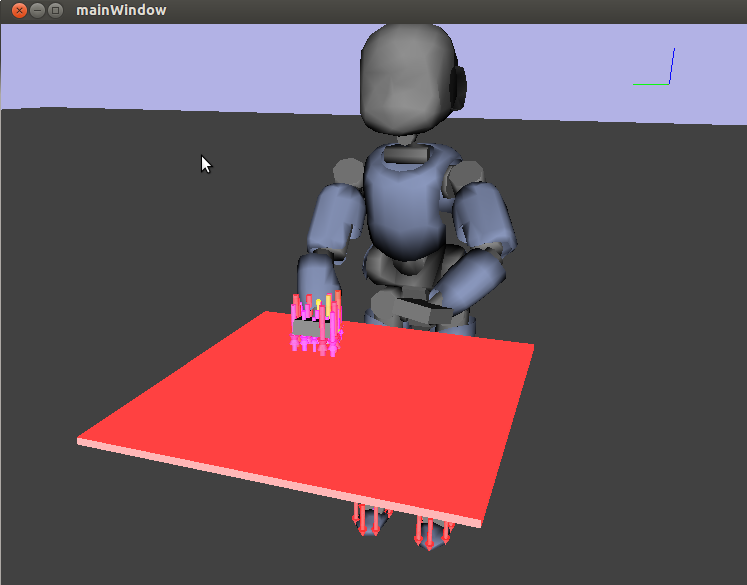
\includegraphics[width=0.3\hsize]{images/s5.png}
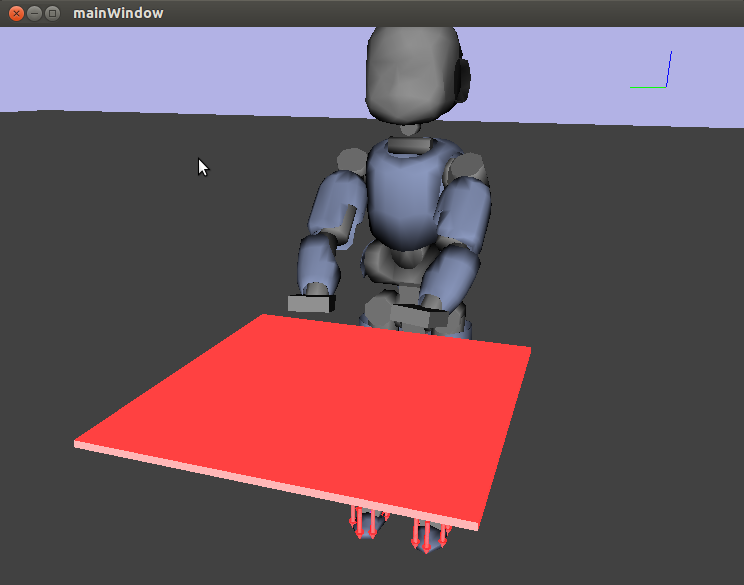
\includegraphics[width=0.3\hsize]{images/s6.png}
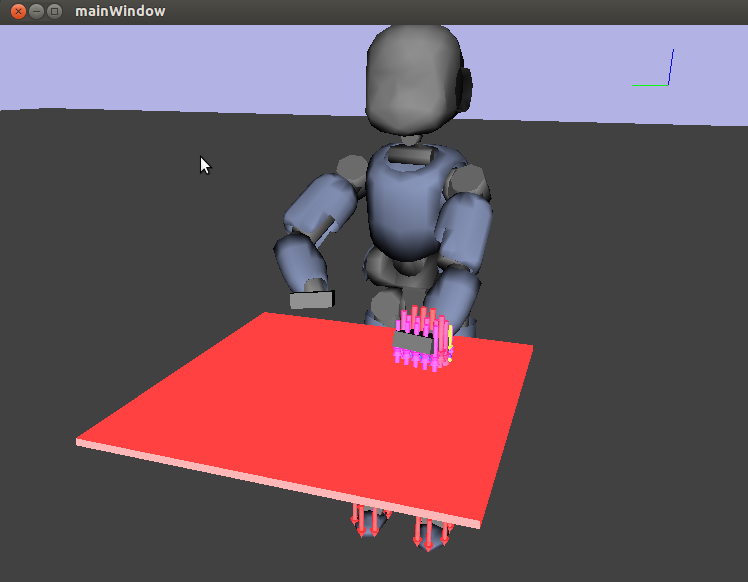
\includegraphics[width=0.3\hsize]{images/s4.png}

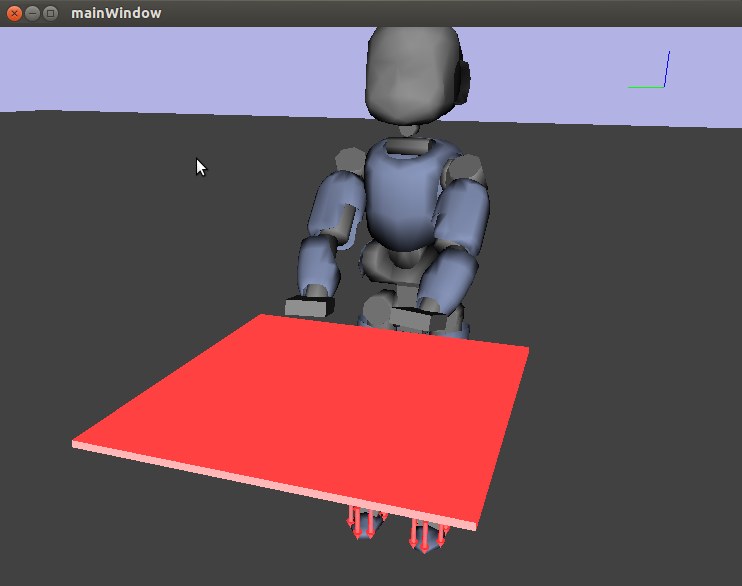
\includegraphics[width=0.3\hsize]{images/s3.png}
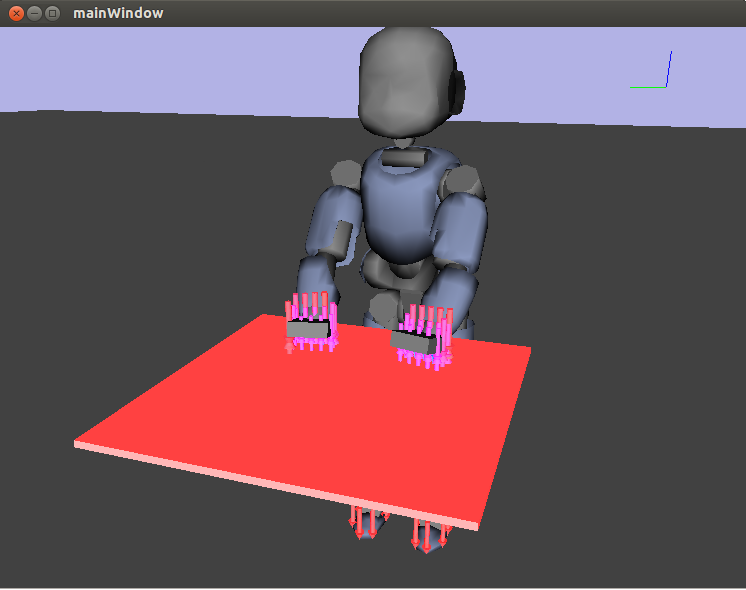
\includegraphics[width=0.3\hsize]{images/s2.png}
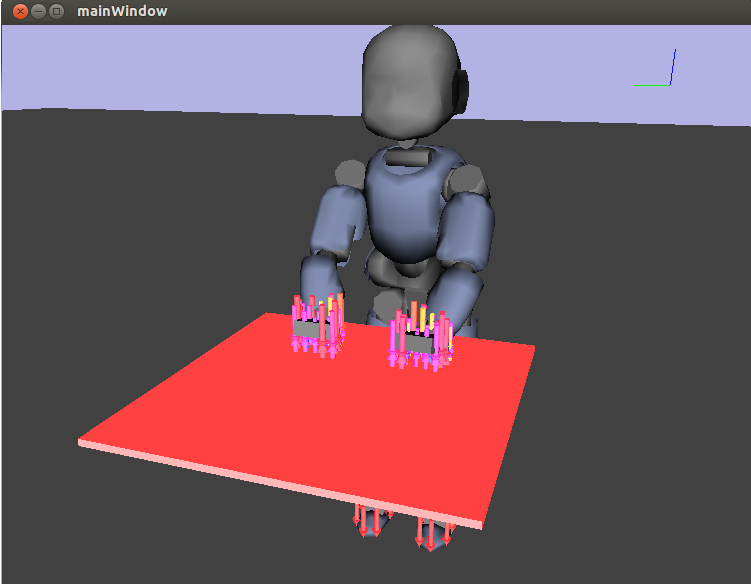
\includegraphics[width=0.3\hsize]{images/s1.png}
\end{center}
\caption{Screenshots of the validation scenario simulated in XDE.}
\label{fig:xde}
\end{figure*}

\subsubsection{Formulating the control problem (T3.2)}

The work performed during year one by UPMC to achieve T3.2 has led to the definition of what a task can be considered to be in the context of the reactive formulation of a multi-task whole body control problem. Among the different characteristics of a task (physical frame, task variable, forward model, desired target trajectory, local controller, priority), the notion of task priority has been largely modified with respect to the classical lexicographic task ordering met in the robotics literature and which is particularly appropriate for cascade resolution approaches such as the one recently proposed in \cite{escande2012}. A partial order has been defined such that task priorities can be described for any pair of task $i$ and $j$. This leads to a richer formulation which includes the original one but is also particularly appropriate for describing task insertion and removal processes as well as priority switching between tasks. Further more, this new prioritization paradigm provides a unique way of defining strict and soft hierarchies between tasks. Associated to this work, the notion  of generalized task projector has been introduced. Each task is associated to a projector which is built based on the tasks priorities. The interest of this projector is that it filters the joint space motion associated to a task so that all priorities are respected, being them soft or strict. Details regarding this work are provided in \cite{liu2013}.

Within this task also IIT contributed with the definition of a software abstraction layer, named wholeBodyInterface (\url{http://wiki.icub.org/codyco/dox/html/namespacewbi.html}). This software library defines the interface to access and control the robot  whole-body. Therefore the wholeBodyLibrary structures the control problem and their definition. Currently the library has been been implemented for both the iCub and the Gazebo iCub simulator.  

\subsubsection{Solving the local control problem (T3.3)}

Associated to the new task formulation proposed in T3.2, the control problem has been formulated by UPMC as an LQP which can be solved by any convex optimization solver dealing with linear constraints. Despite the task hierarchy, the introduction of a generalized task projector per task allows to solve only one LQP. This can be done by introducing as many virtual joint space variables as the number of tasks and using the generalized projector of each task in the expression of the constraints. The resulting problem can be solved by standard convex optimization tools and the cost of introducing virtual joint space variables is compensated for by the fact that only one optimization problem has to be solved. Details regarding this work are provided in \cite{liu2013}.

In the meantime, TUD has proposed to explore optimization methods for solving local control problems that do not require the explicit inversion of any model of the system.  During year one, TUD investigated Bayesian optimization methods that were applied to bipedal locomotion tasks.  One of the key challenges in robotic bipedal locomotion is finding gait parameters that optimize a desired performance criterion, such as speed, robustness or energy efficiency. Typically, gait optimization requires extensive robot experiments and specific expert knowledge. During year one, TUD demonstrated that  data-driven machine learning methods based on Bayesian optimization can be used to automate and speed up the process of gait optimization. These Bayesian optimization methods were used to efficiently find gait parameters that optimize the desired performance metric on a real bipedal walker \cite{calandra2014} and \cite{calandra2014b}.
    

\subsubsection{Bootstrapping and validating the control approach in rigid world and compliant cases (T3.4)}

During year one, UPMC has explored the contribution of MPC approaches to handle the postural balancing problem under varying contact conditions. The hybrid nature of the problem, where varying contact conditions can be accommodated either by adapting the internal forces distribution given a set of contact or by modifying the set of contacts itself, requires control approaches where the desired task trajectories performed through the local, reactive, whole-body controller have to be optimally planned ahead of time in order to provide robust behaviors. The contributions in this domain are mostly related to the work of A. Ibanez \cite{ibanez2013}, \cite{ibanez2014-icra} and \cite{ibanez2014-ark}. The originality of theses contributions lies in:
\begin{itemize}
	\item an augmented ZMP model including external forces exerted directly on indirectly on the center of mass;
	\item a distributed optimization approach that provides a way of generating reference trajectories for the center of mass representing a good compromise given some antagonistic balance and task;
	\item a non scripted foot step placement optimization.
\end{itemize}

UPMC also partially contributed with an experimental study about human behavior during physical contact with the robot. The protocol was registered and obtained the approval of the ethics committee CERES (Conseil d’\'evaluation \'ethique pour les recherches en sant\'e), from University Paris-Decartes. \footnote{Ivaldi et al., "Engagement during human-humanoid interaction", IRB N. 20135200001072.}
The purpose of the experiments is to collect a database of behaviors of experts and naive people interacting physically with the iCub to accomplish a cooperative task. The collected data also include locations of contacts (retrieved through the tactile skin), applied force, robot mouvements: they will be used to study adaptation to human intention during human-robot physical contacts.
    
In the meantime, TUD investigated the interchange of forces during cooperative tasks between humans and robots \cite{berger2013}. Three example scenarios are illustrated in Figure \ref{fig:interaction_tasks}. In such tasks, typically an exchange of forces takes place whenever the interacting agents make contact. Sometimes, forces are even exchanged through an object that is manipulated by both agents, e.g., through a box that is lifted. For a successful execution of such joint physical activities, a robot needs to accommodate for the external forces exerted by a human. To this end, we developed a machine learning approach for identifying external influences and guidance information from humans. During behavior execution by a robot, predictions from a statistical sensor model are continuously compared with stability parameters derived from current sensor readings. Differences between predicted and measured values exceeding the variance of the statistical model are interpreted as perturbations caused by a human and are used to adapt the robot's behavior.
    
\begin{figure}[!ht]
\centering
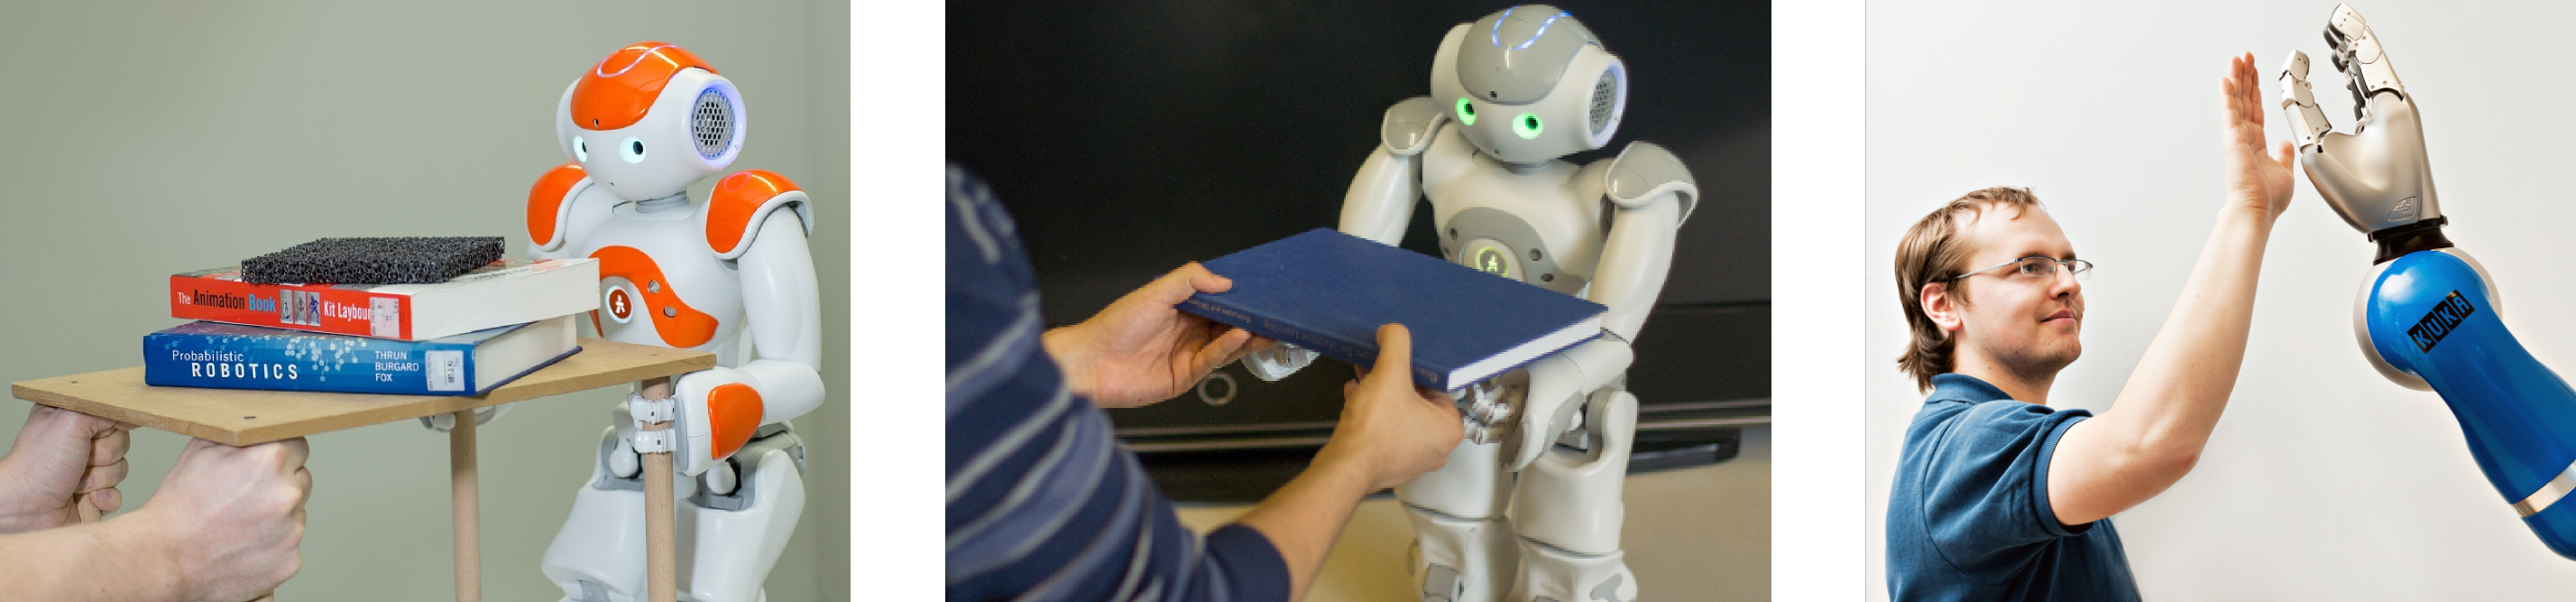
\includegraphics[width=\textwidth]{./images/interaction_wp3.png}
%\label{fig:subfig2}
 \caption{Illustration of three human robot interaction tasks, where an exchange of forces takes place investigated by TUD during year one.
}
\label{fig:interaction_tasks}
\end{figure}

\subsubsection{Deviations from workplan}  

The PM expenses for WP3 after one year of project are globally conform to the planned one. The observed deviations are related to the fact that tasks 3.3 and 3.4 spans the overall duration of the project and the contribution of some of the partners are expected in the 2nd, 3rd and 4th year.

%\emph{\color{red}[For work package 3 (UPMC) provide the following information:]}
%\begin{itemize}
%\item[-] \emph{\color{red}[A summary of progress towards objectives and details for each task;]}
%\item[-] \emph{\color{red}[Highlight clearly significant results;]}
%\item[-] \emph{\color{red}[If applicable, explain the reasons for deviations from Annex I and their impact on other tasks as well as on available resources and planning;]}
%\item[-] \emph{\color{red}[If applicable, explain the reasons for failing to achieve critical objectives and/or not being on schedule and explain the impact on other tasks as well as on available resources and planning (the explanations should be consistent with the declaration by the project coordinator) ;]}
%\item[-] \emph{\color{red}[a statement on the use of resources, in particular highlighting and explaining deviations between actual and planned  person-months per work package and per beneficiary in Annex 1 (Description of Work);]}
%\item[-] \emph{\color{red}[If applicable, propose corrective actions.]}
%\end{itemize}

\subsubsection{Resources}

\begin{center}
\begin{tabular}{|l|l|l|l|l}
\cline{1-4}
 & Planned PM for year 1 & Actual PM & Comment & \\ \cline{1-4}
IIT & 2 & 2 &  &  \\ \cline{1-4}
TUD & 6 & 4.6 &  &  \\ \cline{1-4}
UPMC & 22.5 & 22 &  &  \\ \cline{1-4}
UB & 2.5 & ? &  &  \\ \cline{1-4}
JSI & 1 & 0 &  &  \\ \cline{1-4}
\end{tabular}
\end{center}

\subsection{Work package 4 progress}

\subsubsection{Generalizing and Improving Elementary Tasks with Contacts (T4.3)}

In this task, we aim to generate new skills from data, where elementary skills 
are acquired by imitation learning and transferred to novel situations using 
dynamic systems. During year one, TUD developed a novel representation of 
movement primitives that can be used for imitation learning from noisy observations.
Uncertainty of observed trajectories is explicitely modeled and used to generate new skills.
This movement representation has state-of-the-art capabilities in generalization, 
coupling between the degrees of freedom of the robot, and moreover, 
a time varying feedback controller can be derived in closed form. 
These features are partially illustrated in Figure \ref{fig:promps}.
This work was published
last year at the highly competitive conference on neural information processing (NIPS) 
[Paraschos, A. and  Daniel, C. and  Peters, J. and Neumann, G, 2013].

\begin{figure}[!ht]
\centering
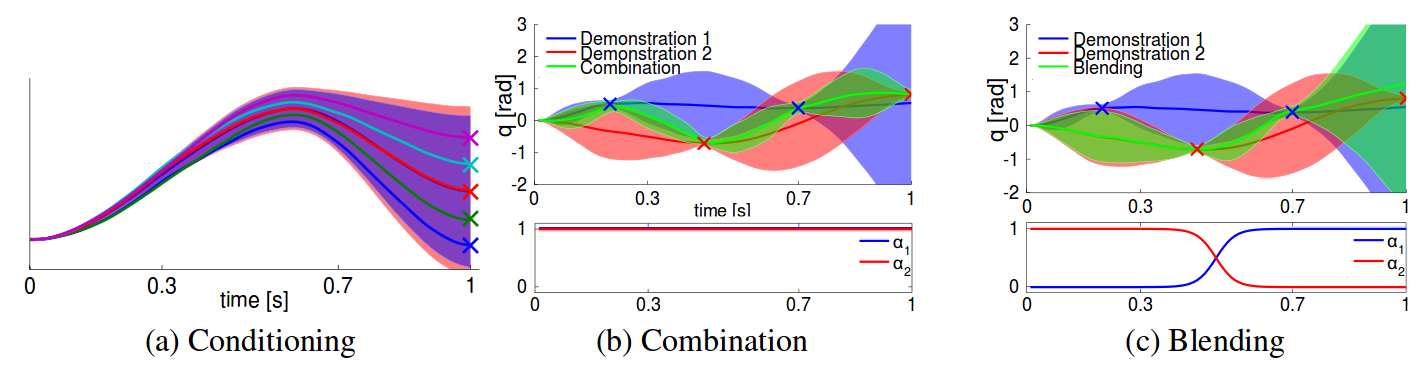
\includegraphics[width=\textwidth]{./images/ProMPs.png}
%\label{fig:subfig2}
 \caption{(a)
Conditioning on different target states. The blue shaded area represents the learned
trajectory distribution. We condition on different target positions, indicated by the ‘x’-markers. The
produced trajectories exactly reach the desired targets while keeping the shape of the demonstrations.
(b)
Combination of two ProMPs. The trajectory distributions are indicated by the blue and red
shaded areas. Both primitives have to reach via-points at different points in time, indicated by
the ‘x’-markers. We co-activate both primitives with the same activation factor. The trajectory
distribution generated by the resulting feedback controller now goes through all four via-points.
(c)
Blending of two ProMPs. We smoothly blend from the red primitive to the blue primitive. The
activation factors are shown in the bottom. The resulting movement (green) first follows the red
primitive and, subsequently, switches to following the blue primitive.
}
\label{fig:promps}
\end{figure}

In another work, published at the international conference on humanoid robots (HUMANOIDS), 
TUD demonstrated that this probabilistic approach for trajectory generation
has superior performance against deterministic policies. The use of
probability distributions over the trajectories increased significantly
 the generalization properties, which was evaluated on a high dimensional table
tennis scenario [Paraschos, A. and  Neumann, G and  Peters, J., 2013]. 
In the future work, we plan to incorporate external torque signals to initiate, 
maintain, and terminate contacts.

TUD also investigated how to learn human robot interaction through imitation. We presented a new approach to robot learning that allows anthropomorphic robots to learn a library of interaction skills from demonstration [H Ben Amor, D Vogt, M Ewerton, E Berger, B Jung and J Peters, 2014]. Traditional approaches to modeling interactions assume a pre-specified symbolic representation of the available actions. For example, they model interactions
in terms of commands such as \emph{wait}, \emph{pick-up}, and \emph{place}. Instead of such a top-down approach, we focused on learning responsive behavior in a bottom-up fashion using a trajectory based approach. The key idea behind our approach is that the observation of human-human collaborations can provide rich information specifying how and when to interact
in a particular situation. For example, by observing how two human workmen collaborate on lifting a heavy box, a robot could use machine learning algorithms to extract an
interaction model that specifies the states, movements, and situational responses of the involved parties. In turn, such a model can be used by the robot to assist in a similar lifting task. Our approach is as an extension of imitation learning to multi-agent scenarios, in which the behavior and the mutual interplay between two agents is imitated

\begin{figure}[!ht]
\centering
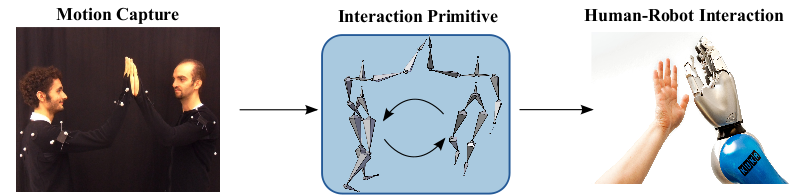
\includegraphics[width=\textwidth]{./images/newoverview.png}
%\label{fig:subfig2}
 \caption{Illustration of the developed interaction primitives that allows to infer the behavior of the interacting partner.
}
\label{fig:interaction_primitives}
\end{figure}

We further extended the above approach by introducing \emph{Interaction Primitives} in [Ben Amor, H.; Neumann, G.; Kamthe, S.; Kroemer, O.; Peters, J., 2014]. Interaction primitives build on the framework of dynamic motor primitives (DMPs) by maintaining a distribution over the parameters of the DMP. With this distribution, we can learn the inherent correlations of cooperative activities which allow us to infer the behavior of the partner and to participate in the cooperation. A conceptual overview is sketched in Figure \ref{fig:interaction_primitives}. A learned Interaction Primitive can be used by a robot to (1) predict the human's next action in the current context, (2) identify the optimal response, (3) synchronize the movement with the human partner.

In the meantime, demonstration-based learning of "optimal trajectories" and stable controllers has been addressed by UPMC, in particular in \cite{stulp2013} where a general, flexible, and compact representation of parameterizable skills is proposed. This work generalizes the standard Dynamic Motor Primitive formulation in \cite{ijspeert2013} and proposes a novel DMP formulation for parametrized skills, based on additionally passing task parameters to the DMP function approximator. This generalizes previous approaches, in particular those which train and execute parametrized skills with two separate regressions. Learning the function approximator with one regression in the full space of phase and tasks parameters allows for more compact models, and the flexible use of different function approximator implementations such as LWPR and GPR, as we demonstrated on the Meka and iCub humanoids robots.


\subsubsection{Resources}

\begin{center}
\begin{tabular}{|l|l|l|l|l}
\cline{1-4}
 & Planned PM & Actual PM & Comment & \\ \cline{1-4}
IIT & 9.3 &  &  &  \\ \cline{1-4}
TUD & 10.4 & 8 &  &  \\ \cline{1-4}
UPMC & 5 &  &  &  \\ \cline{1-4}
UB & 3 &  &  &  \\ \cline{1-4}
JSI & 2.5 &  &  &  \\ \cline{1-4}
\end{tabular}
\end{center}

\subsubsection{Deviations from workplan} 

No significant deviations. 

\subsection{Work package 5 progress}

The activities in WP5 are divided into four tasks corresponding to the four years project duration. As a result, during the first year CoDyCo results concentrate on T5.1. The main result consist in the implementation of the validation scenario consisting of the balancing on different type of rigid contacts.

\subsubsection{Scenario 1: iCub balancing on multiple rigid contacts (T5.1)}

The main contributions to T5.1 have been presented in ``D5.1 Scientific report on validation scenario 1: balancing on multiple rigid contact points.'' which discusses the technical implementation of the first year validation scenario (see \url{https://github.com/robotology-playground/codyco-deliverables/tree/master/D5.1/pdf}). The software developed for the scenario implementation is released with an open-source license and distributed through github (\url{https://github.com/robotology/codyco} ). The main software activities include: a module to identify the whole-body motor transfer functions (\url{https://github.com/robotology/codyco/tree/master/src/modules/motorFrictionIdentification}), a module for estimating whole-body internal (joint torques) and external (contact) forces (\url{https://github.com/robotology/codyco/tree/master/src/modules/motorFrictionIdentification}), a module for whole-body joint torque control (\url{https://github.com/robotology/codyco/tree/master/src/modules/jointTorqueControl}), a C++ library that implements the wholeBodyInterface in simulink (\url{https://github.com/robotology/codyco/tree/master/src/simulink}).

\subsubsection{Deviations from workplan}  

The original work plan have foreseen contacts at feet, hands, back, buttocks, arms and legs. The final validation scenario will only include possible contacts at hands and feet. This simplification is mainly due to the fact that at he end of the CoDyCo first year the iCub does not yet include tactile sensing on the back, legs and buttocks. These sensors will be soon included in the iCub and the CoDyCo software is already designed to include this information. 

%\begin{itemize}
%\item[-] \emph{\color{red}[A summary of progress towards objectives and details for each task;]}
%\item[-] \emph{\color{red}[Highlight clearly significant results;]}
%\item[-] \emph{\color{red}[If applicable, explain the reasons for deviations from Annex I and their impact on other tasks as well as on available resources and planning;]}
%\item[-] \emph{\color{red}[If applicable, explain the reasons for failing to achieve critical objectives and/or not being on schedule and explain the impact on other tasks as well as on available resources and planning (the explanations should be consistent with the declaration by the project coordinator) ;]}
%\item[-] \emph{\color{red}[a statement on the use of resources, in particular highlighting and explaining deviations between actual and planned  person-months per work package and per beneficiary in Annex 1 (Description of Work);]}
%\item[-] \emph{\color{red}[If applicable, propose corrective actions.]}
%\end{itemize}

\subsubsection{Resources}

Resources were used as expected.

\begin{center}
\begin{tabular}{|l|l|l|l|l}
\cline{1-4}
 & Planned PM for year 1 & Actual PM & Comment & \\ \cline{1-4}
IIT & 12 & 12 &  &  \\ \cline{1-4}
UPMC & 1 & 0.33 &  &  \\ \cline{1-4}
\end{tabular}
\end{center}

\subsection{Work package 6 progress}

Activities within work package 6 achieved the expected results both in terms of administrative activities and management activities. As a major result, the software repository was successfully implemented thanks to novel versioning tool (git) and social coding website (\url{https://github.com}).

\subsubsection{Administrative coordination (T6.1)}
Administration was successfully coordinated by Chiara Andreoli at IIT. The major activity concerned an amendment that the CoDyCo consortium asked the main reason being the fact that Serena Ivaldi, initially hired by UPMC was recently hired by TUD. Part of the administrative coordination activities were also conducted during three main meetings: the kick-off meeting (Genoa, April 5th, 2013), the simulators meeting (Paris, June 5th, 2013) and the midyear meeting (Paris, November 21st-22nd, 2013). Details on the meetings can be found in the CoDyCo website (\url{http://www.codyco.eu}).

\subsubsection{Software repository implementation (T6.2)}

A github software repository was set up \url{https://github.com/robotology/codyco} and the contribution from the different developers can be directly checked in the website. Relevant information can be found also in ``D6.1 Website and repository online'' available here: \url{https://github.com/robotology-playground/codyco-deliverables/tree/master/D6.1/pdf}.

\subsubsection{Resources}

Resources were used as follows.

\begin{center}
\begin{tabular}{|l|l|l|l|l}
\cline{1-4}
 & Planned PM for year 1 & Actual PM & Comment & \\ \cline{1-4}
IIT        & 1 & 1 &  &  \\ \cline{1-4}
TUD    & ? & ? &  &  \\ \cline{1-4}
UPMC & ? & ? &  &  \\ \cline{1-4}
JSI       & ? & ? &  &  \\ \cline{1-4}
UB       & ? & ? &  &  \\ \cline{1-4}
\end{tabular}
\end{center}

%\begin{itemize}
%\item[-] \emph{\color{red}[A summary of progress towards objectives and details for each task;]}
%\item[-] \emph{\color{red}[Highlight clearly significant results;]}
%\item[-] \emph{\color{red}[If applicable, explain the reasons for deviations from Annex I and their impact on other tasks as well as on available resources and planning;]}
%\item[-] \emph{\color{red}[If applicable, explain the reasons for failing to achieve critical objectives and/or not being on schedule and explain the impact on other tasks as well as on available resources and planning (the explanations should be consistent with the declaration by the project coordinator) ;]}
%\item[-] \emph{\color{red}[a statement on the use of resources, in particular highlighting and explaining deviations between actual and planned  person-months per work package and per beneficiary in Annex 1 (Description of Work);]}
%\item[-] \emph{\color{red}[If applicable, propose corrective actions.]}
%\end{itemize}

\subsection{Work package 7 progress}

Dissemination and exploitation activities included the participation to international events addressed to both commercial and academic institutions. A preliminary exploitation plan was delineated and reported in the deliverable D7.1.

\subsubsection{Dissemination activities towards academia, industry, and other users (T7.1)}

Dissemination activities were conducted in three main events: (1) iCub exposition at IROS2014, IEEE International Conference on Robotics and Automation Karlsruhe, May 6 - 10, 2013; (2) iCub exposition at the European Robotics Forum and Innorobo, Lyon 29th March 2013; (3) iCub exposition at the European Robotics Forum, Rovereto 12th-14th of March 2014. The full list of papers published within CoDyCo can be found here: \url{http://codyco.eu/publications-menu}.

\subsubsection{Exploitation plan (T7.2)}

The first year activities on T7.1 and T7.2 are all contained in ``D7.1 Dissemination and exploitation plan'' available here: \url{https://github.com/robotology-playground/codyco-deliverables/tree/master/D7.1/pdf}.

\subsubsection{Management of IPR (T7.3)}

No activities to be reported during the first year on this task in consideration of the fact that the task started at the very end of the first year. As a minor starting activity the consortium circulated a list containing each partner responsible contact person for the IPR management. This list is contained in ``D7.1 Dissemination and exploitation plan'' available here: \url{https://github.com/robotology-playground/codyco-deliverables/tree/master/D7.1/pdf}.

\subsubsection{Dissemination of a database of human motion with contacts (T7.4)}

During the first year of CoDyCo, IIT completed the task of setting up a database for storing both human and robot datasets. The details on the database are reported in ``D7.2 Standard database with support materials'' available here \url{https://github.com/robotology-playground/codyco-deliverables/tree/master/D7.2/pdf}. 

\subsubsection{Resources}

Resources were used as follows.

\begin{center}
\begin{tabular}{|l|l|l|l|l}
\cline{1-4}
 & Planned PM for year 1 & Actual PM & Comment & \\ \cline{1-4}
IIT        & 1 & 1 &  &  \\ \cline{1-4}
TUD    & ? & ? &  &  \\ \cline{1-4}
UPMC & ? & ? &  &  \\ \cline{1-4}
JSI       & ? & ? &  &  \\ \cline{1-4}
UB       & ? & ? &  &  \\ \cline{1-4}
\end{tabular}
\end{center}

%\begin{itemize}
%\item[-] \emph{\color{red}[A summary of progress towards objectives and details for each task;]}
%\item[-] \emph{\color{red}[Highlight clearly significant results;]}
%\item[-] \emph{\color{red}[If applicable, explain the reasons for deviations from Annex I and their impact on other tasks as well as on available resources and planning;]}
%\item[-] \emph{\color{red}[If applicable, explain the reasons for failing to achieve critical objectives and/or not being on schedule and explain the impact on other tasks as well as on available resources and planning (the explanations should be consistent with the declaration by the project coordinator) ;]}
%\item[-] \emph{\color{red}[a statement on the use of resources, in particular highlighting and explaining deviations between actual and planned  person-months per work package and per beneficiary in Annex 1 (Description of Work);]}
%\item[-] \emph{\color{red}[If applicable, propose corrective actions.]}
%\end{itemize}

\bibliographystyle{IEEEtran}
% \bibliography{IEEEabrv,yearReport_WP3,all-ias-publications}
\bibliography{firstYearReport_WP3,firstYearReport_WP2}

\end{document}

%%% Local Variables:
%%% mode: latex
%%% TeX-master: t
%%% save-place: t
%%% End:
